\documentclass{amsart}
\usepackage[utf8]{inputenc}
\usepackage[usefamily=sage]{pythontex} 
\usepackage{float}
\usepackage{tikz}
\usetikzlibrary{calc}
\usepackage[most]{tcolorbox}
\usepackage[margin = 2cm]{geometry}
\usepackage{graphicx}
\usetikzlibrary{3d}
\usepackage{tikz-3dplot}

\newtheorem{ejer}{Ejercicio}
\def\r{\mathbb{R}}





\title{ AMD Curso 2023-2024. Prácticas de la Semana 13. Geometría Afín}

\begin{document}

\maketitle

\begin{tcolorbox}[colback = orange!60!white,title = Cuestiones teóricas previas]
Una aplicación $f:\mathcal{A}^n(\mathbb R) \to \mathcal{A}^n(\mathbb R)$ se dice { \bf afín} si existen una matriz $A$ de orden $n\times n$ y un punto $Q\in \mathbb R^n$ tales que $f(P)=AP+Q$, lo cual se expresa con matrices del siguiente modo: 
%Su expresión matricial asociada es:
$$\left[ \frac{1}{f(P)}\right]=\left[ \frac{ \ 1 
  \ | \  0 \ }{Q \ | \ A}\right] \left[ \frac{1}{Q}\right]$$
Entre las aplicaciones afines (en el plano y en el espacio), nos interesan especialmente un grupo de transformaciones geométricas que reciben el nombre de  {\bf transformaciones afines}, y son las siguientes:
\begin{itemize}
\item Transformaciones afines en el plano:
\begin{itemize}
\item Giro alrededor de un punto.
\item Proyección ortogonal sobre una recta
\item Simetría ortogonal sobre una recta
\item Homotecia
\end{itemize}
\item Transformaciones afines en el espacio:
\begin{itemize}
\item Giro alrededor de un recta.
\item Proyección ortogonal sobre una recta o un plano
\item Simetría ortogonal sobre una recta o un plano
\item Homotecia
\end{itemize}
\end{itemize}
La matriz $M_T$ asociada a cada una de estas transformaciones $T$ tiene una forma especialmente sencilla (su expresión canónica) porque se toma respecto de un sistema de referencia afín $R$ que se adapta especialmente bien a lo que hace la transformación afín $T$. Por ejemplo, si $T=G_{\alpha}$ es un giro en el plano de ángulo $\alpha$, centrado en el punto $Q$, entonces $$R=\left[ \frac{ \ 1 
  \ | \  0 \ }{Q \ | \ C}\right],$$
donde $C$ es la base canónica de $\mathbb{R}^2$, y 
$$M_{G_{\alpha}}= \left[\begin{array}{ccc}  1 & 0 & 0 \\ 0& \cos \alpha & -\sin \alpha \\  0& \sin \alpha & \cos \alpha\end{array}\right]$$

Entonces la matriz asociada, $M(T)$, respecto del sistema de referencia canónico del espacio afín,  se expresa en términos de  $M_{T}$ como:
$$M(T)=RM_{T}R^{-1}$$
En lo sucesivo, denotaremos como $M_{RR}(T)$ a la matriz $M_T$ para dejar constancia, en cada caso, de cuál es el sistema de referencia afín especial, $R$, que se ha usado para obtener la expresión canónica de la transformación $T$ -y que luego usamos para obtener la matriz $M(T)$, que es la asociada a $T$ respecto del sistema de referencia canónico de $\mathcal{A}^n(\mathbb R)$.
%También podemos usar un sistema de referencia afín general (normalmente, tomamos una base vectorial ortogonal u ortonormal $B$ y un punto $Q$),
%$$R_1=\left[ \frac{ \ 1 
%  \ | \  0 \ }{Q \ | \ B}\right]$$
%Y la matriz asociada para ese sistema de referencia será:
%$$M_{R1R1}(T)=R_1M_{T}R_1^{-1}$$

\end{tcolorbox} 
\newpage

\begin{ejer}	
\textcolor{blue}{\begin{enumerate} 
\item[a)] Calcula la matriz de la aplicación af\'{i}n $g:\mathcal{A}^2(\mathbb R) \to \mathcal{A}^2(\mathbb R)$ correspondiente al {\sc giro} de $30^\circ$ alrededor del punto 
$\left( \begin{array}{r} 2  \\ -1 \end{array} \right)$.
\item[b)] Sea $C \subseteq \mathcal{A}^2(\mathbb R)$ el hex\'agono regular centrado en el punto $\left( \begin{array}{r} 4  \\ 4 \end{array} \right)$ tal que uno de sus v\'ertices
es el punto $\left( \begin{array}{r} 5  \\ 4 \end{array} \right)$. Calcula todos los v\'ertices de $C$ y $g(C)$. Dibuja los hexágonos $C$, $g(C)$ y las líneas que unen los centros de los hexágonos con el centro de giro.
\end{enumerate}}
\end{ejer}

{\it Solución:}

% Escribe tu solución para el ejercicio 1

a.

\begin{sageblock}
R = matrix(RR, [[1, 0, 0], [2, 1, 0], [-1, 0, 1]])
alpha = pi/6
MRRg = matrix(RR, [[1, 0, 0], [0, cos(alpha), -sin(alpha)], [0, sin(alpha), cos(alpha)]])

Mg = R * MRRg * R^-1
\end{sageblock}

$$
	R = \begin{bmatrix}
		1 & 0 & 0 \\
		2 & 1 & 0 \\
		-1& 0 & 1
	\end{bmatrix}
$$

$$
	M_{RR}(g) = \begin{bmatrix}
		1 & 0 & 0 \\
		0 & cos(30) & -sin(30) \\
		0 & sin(30) & cos(30)
	\end{bmatrix}
$$

$$
	M = R M_{RR}(g) R^{-1} = \sage{Mg}
$$

b.

\begin{sageblock}
R1 = matrix(RR, [[1, 0, 0], [4, 1, 0], [4, 0, 1]])

b = pi/3
MRRg = matrix(RR, [[1, 0, 0], [0, cos(b), -sin(b)], [0, sin(b), cos(b)]])

Mg1 = R1 * MRRg * R1^-1

C = [Mg1^i * vector(RR, [1, 5, 4]) for i in range(6)]
gC = [Mg * v for v in C]
gCo = (Mg * vector(RR, [1, 4, 4]))[1:]

C = [v[1:] for v in C]
gC = [v[1:] for v in gC]
\end{sageblock}

%\begin{verbatim}
\begin{sagesub}
\begin{center}
\begin{tikzpicture}[scale = 1,
cara1/.style={thick, color = blue, fill opacity = 0.3, fill = blue!20},
cara2/.style={thick, color = red, fill opacity = 0.3, fill = red!20},
]
\draw[->,thick,gray] (-1,0) -- (5.5,0); % Eje X
\draw[->,thick,gray] (0,-2.5) -- (0,5.5); % Eje Y

\draw[cara1] !{C[0]} -- !{C[1]} -- !{C[2]} -- !{C[3]} -- !{C[4]} -- !{C[5]} -- cycle;
\draw[cara2] !{gC[0]} -- !{gC[1]} -- !{gC[2]} -- !{gC[3]} -- !{gC[4]} -- !{gC[5]} -- cycle;
\draw[black] (2,-1) -- (4,4);
\draw[black] (2,-1) -- !{gCo};
\end{tikzpicture}
\end{center}
\end{sagesub}
%\end{verbatim}


% Fin del Ejercicio 1

\newpage


\begin{ejer}
\textcolor{blue}{Sea $r \subseteq \mathcal{A}^2(\mathbb R)$ la recta que pasa por los puntos $\left( \begin{array}{r} -1  \\ 0 \end{array} \right)$ y $\left( \begin{array}{r} 2  \\ 2 \end{array} \right)$.
\begin{enumerate} 
\item[a)] Calcula las matrices de las aplicaciones afines $p,s:\mathcal{A}^2(\mathbb R) \to \mathcal{A}^2(\mathbb R)$ correspondientes a la {\sc proyección} y a la {\sc simetría} 
respecto de $r$. 
\item[b)] Sea $C \subseteq \mathcal{A}^2(\mathbb R)$ el cuadrado centrado en el punto $\left( \begin{array}{r} 3  \\ -3 \end{array} \right)$ y con uno de sus vértices
en $\left( \begin{array}{r} 4  \\ -2 \end{array} \right)$. 
\begin{itemize}
\item Calcula todos los vértices de $C$ y $s(C)$.
\item Dibuja $r$, $C$, $s(C)$, $p(C)$ y las líneas que unen los vértices del cuadrado $C$ con su simétrico $s(C)$.
\end{itemize}
\end{enumerate}}
\end{ejer}

{\it Solución:}

% Escribe tu solución para el ejercicio 2

\begin{sageblock}
pr1 = vector(RR, [-1, 0])
pr2 = vector(RR, [2, 2])
vr = (pr2 - pr1)
u1 = vr.normalized()
u2 = vector(RR, [vr[1], -vr[0]]).normalized()

R = matrix(RR, [[1, 0, 0], [pr1[0], u1[0], u2[0]], [pr1[1], u1[1], u2[1]]])
MRRp = matrix(RR, [[1, 0, 0], [0, 1, 0], [0, 0, 0]])
MRRs = matrix(RR, [[1, 0, 0], [0, 1, 0], [0, 0, -1]])

Mp = R * MRRp * R^-1
Ms = R * MRRs * R^-1
\end{sageblock}

a.

$$
	R = \sage{R}
$$

$$
	M_p = \sage{Mp}
$$

$$
	M_s = \sage{Ms}
$$

b.

\begin{sageblock}
R = matrix(RR, [[1, 0, 0], [3, 1, 0], [-3, 0, 1]])

a = pi/2
MRRg = matrix(RR, [[1, 0, 0], [0, cos(a), -sin(a)], [0, sin(a), cos(a)]])
Mg = R * MRRg * R^-1

cp0 = vector(RR, [1, 4, -2])

C = [Mg^i * cp0 for i in range(4)]
sC = [Ms * v for v in C]
pC = [Mp * v for v in C]

C = [v[1:] for v in C]
sC = [v[1:] for v in sC]
pC = [v[1:] for v in pC]
\end{sageblock}

\begin{sagesub}
\begin{center}
\begin{tikzpicture}[scale = 1,
cara1/.style={thick, color = blue, fill opacity = 0.3, fill = blue!20},
cara2/.style={thick, color = red, fill opacity = 0.3, fill = red!20},
]
\draw[->,thick,gray] (-1,0) -- (5.5,0); % Eje X
\draw[->,thick,gray] (0,-2.5) -- (0,5.5); % Eje Y

\draw[->,thick,red] !{pr1} -- !{pr2}; % recta

\draw[->,thick,yellow] !{pr1} -- !{pr1 + u1}; % recta
\draw[->,thick,yellow] !{pr1} -- !{pr1 + u2}; % recta

\draw[black] (3, -3) circle (2pt);
\draw[black] (4, -2) circle (2pt);

\draw[cara1] !{C[0]} -- !{C[1]} -- !{C[2]} -- !{C[3]} -- cycle;
\draw[cara1] !{sC[0]} -- !{sC[1]} -- !{sC[2]} -- !{sC[3]} -- cycle;
\draw[cara1] !{pC[0]} -- !{pC[1]} -- !{pC[2]} -- !{pC[3]} -- cycle;
%\draw[black] (2,-1) -- (4,4);
\end{tikzpicture}
\end{center}
\end{sagesub}

% Fin del Ejercicio 2

\newpage

\begin{ejer}
\textcolor{blue}{\begin{enumerate} 
\item[a)] Calcula la matriz de la aplicación afín $h:\mathcal{A}^2(\mathbb R) \to \mathcal{A}^2(\mathbb R)$ correspondiente a la {\sc homotecia} con factor $3$
y con centro en el punto $P=\left( \begin{array}{r} 1 \\ 1 \end{array} \right)$.
\item[b)]Sea $C \subseteq \mathcal{A}^2(\mathbb R)$ el triángulo isósceles contenido en el segundo cuadrante que tiene altura $5$ y cuya base 
es el segmento con extremos $\left( \begin{array}{r} -4 \\ 2 \end{array} \right)$ y $\left( \begin{array}{r} -3 \\ 2 \end{array} \right)$. 
\begin{itemize}
\item Calcula todos los vértices de $C$ y $h(C)$. 
\item Dibuja $P$, $C$ y $h(C)$.
\end{itemize}
\end{enumerate}}
\end{ejer}

{\it Solución:}

% Escribe tu solución para el ejercicio 3
a.

\begin{sageblock}
R = matrix(RR, [[1, 0, 0], [1, 1, 0], [1, 0, 1]])
f = 3
MRRh = matrix(RR, [[1, 0, 0], [0, f, 0], [0, 0, f]])

Mf = R * MRRh * R^-1

tp0 = vector(RR, [-4, 2])
tp1 = vector(RR, [-3, 2])
tsv = tp1 - tp0
tsmp = tp0 + tsv/2
tp2 = tsmp + 5 * vector(RR, [-tsv[1], tsv[0]]).normalized()

C = vector(RR, [1, tp0[0], tp0[1]]), vector(RR, [1, tp1[0], tp1[1]]), vector(RR, [1, tp2[0], tp2[1]])
hC = [Mf * v for v in C]

C = [v[1:] for v in C]
hC = [v[1:] for v in hC]
\end{sageblock}

\begin{sagesub}
\begin{center}
\begin{tikzpicture}[scale = 1,
cara1/.style={thick, color = blue, fill opacity = 0.3, fill = blue!20},
cara2/.style={thick, color = red, fill opacity = 0.3, fill = red!20},
]
\draw[->,thick,gray] (-5,0) -- (0,0); % Eje X
\draw[->,thick,gray] (0,0) -- (0,8); % Eje Y

\draw[cara1] !{C[0]} -- !{C[1]} -- !{C[2]} -- cycle;
\draw[cara1] !{hC[0]} -- !{hC[1]} -- !{hC[2]} -- cycle;


\draw[black] (1, 1) circle (2pt);
\end{tikzpicture}
\end{center}
\end{sagesub}

% Fin del Ejercicio 3



\newpage


\begin{ejer}
\textcolor{blue}{Calcula los vértices de un octógono regular en $\mathcal{A}^2(\mathbb{R})$ centrado en el punto $\left[\begin{array}{c}1\\3
\end{array}\right]$, sabiendo que el punto $\left[\begin{array}{c}2\\5
\end{array}\right]$ es un vértice de dicho octógono. Pinta el octógono en color amarillo y sus vértices en color azul.}
\end{ejer}

{\it Solución:}

% Escribe tu solución para el ejercicio 4

\begin{sageblock}
R = matrix(RR, [[1, 0, 0], [1, 1, 0], [3, 0, 1]])

a = pi/4
MRRg = matrix(RR, [[1, 0, 0], [0, cos(a), -sin(a)], [0, sin(a), cos(a)]])
Mg = R * MRRg * R^-1

op0 = vector(RR, [1, 2, 5])

C = [Mg^i * op0 for i in range(8)]
C = [v[1:] for v in C]
\end{sageblock}

\begin{sagesub}
\begin{center}
\begin{tikzpicture}[scale = 1,
cara1/.style={thick, color = yellow, fill opacity = 0.3, fill = yellow!20},
]
\draw[->,thick,gray] (-3,0) -- (5,0); % Eje X
\draw[->,thick,gray] (0,-1) -- (0,7); % Eje Y

\draw[cara1] !{C[0]} -- !{C[1]} -- !{C[2]} -- !{C[3]} -- !{C[4]} -- !{C[5]} -- !{C[6]} -- !{C[7]} -- cycle;

\filldraw[blue] !{C[0]} circle (2pt);
\filldraw[blue] !{C[1]} circle (2pt);
\filldraw[blue] !{C[2]} circle (2pt);
\filldraw[blue] !{C[3]} circle (2pt);
\filldraw[blue] !{C[4]} circle (2pt);
\filldraw[blue] !{C[5]} circle (2pt);
\filldraw[blue] !{C[6]} circle (2pt);
\filldraw[blue] !{C[7]} circle (2pt);

\draw[black] (1, 3) circle (2pt);
\end{tikzpicture}
\end{center}
\end{sagesub}

% Fin del Ejercicio 4


\newpage

\begin{ejer}
\textcolor{blue}{Se dibuja una estrella regular de $5$ puntas con centro en el punto $O_1 = \left[ \begin{array}{r} -4 \\ -1 \end{array} \right]$ y con vértice $A = \left[ \begin{array}{r} -2 \\ 0 \end{array} \right]$. El resto de los vértices se nombran $B, C, D$ y $E$ tal y como indica la figura. Posteriormente, se gira la estrella un ángulo de $48^\circ $ alrededor del punto $P = \left[ \begin{array}{r} -8 \\ 4 \end{array} \right]$ en sentido positivo.}

\begin{figure}[H]
\centering
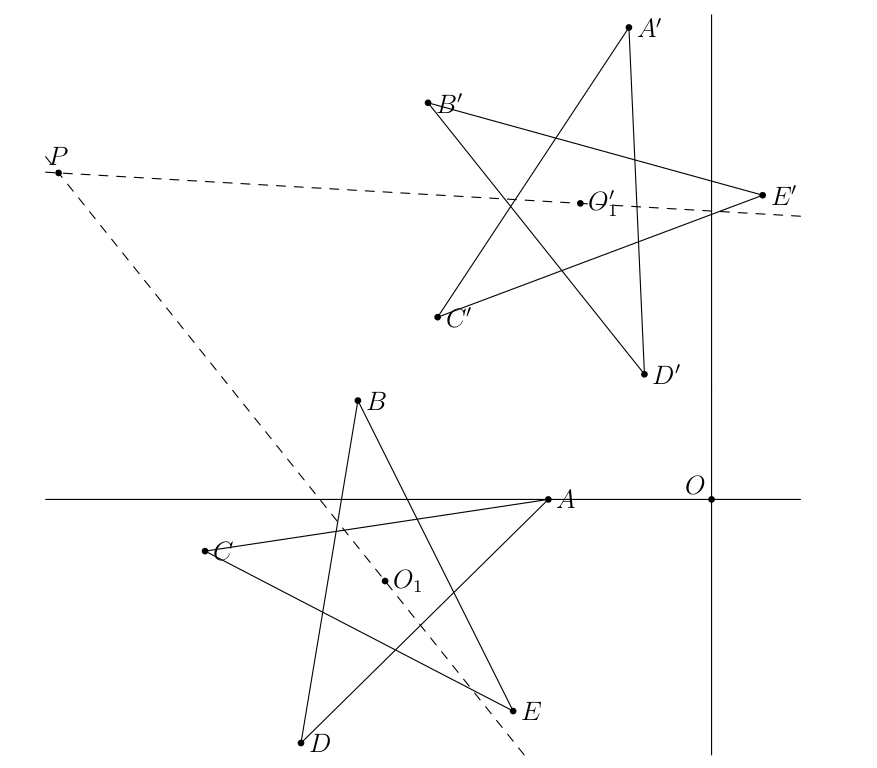
\includegraphics[width = 12cm]{estrella.png}
\end{figure}

\textcolor{blue}{Determinar las coordenadas $x$ e $y$ de los vértices $A,B,C,D,E,A',B',C',D',E'$ y dibuja las estrellas y las líneas que unen los centros de dichas estrellas con el centro de giro.}
\end{ejer}

{\it Solución:}
% Escribe tu solución para el ejercicio 5

\begin{sageblock}
R = matrix(RR, [[1, 0, 0], [-4, 1, 0], [-1, 0, 1]])

a = 2*pi/5
MRRg = matrix(RR, [[1, 0, 0], [0, cos(a), -sin(a)], [0, sin(a), cos(a)]])
Mg = R * MRRg * R^-1

sp0 = vector(RR, [1, -2, 0])

C = [Mg^i * sp0 for i in range(5)]

R = matrix(RR, [[1, 0, 0], [-8, 1, 0], [4, 0, 1]])

a = pi/180 * 48
MRRg = matrix(RR, [[1, 0, 0], [0, cos(a), -sin(a)], [0, sin(a), cos(a)]])
Mg = R * MRRg * R^-1

Cp = [Mg * v for v in C]

C = [v[1:] for v in C]
Cp = [v[1:] for v in Cp]


\end{sageblock}

\begin{sagesub}
\begin{center}
\begin{tikzpicture}[scale = 1,
cara1/.style={thick, color = blue, fill opacity = 0.3, fill = blue!20},
]
\draw[->,thick,gray] (-7,0) -- (1,0); % Eje X
\draw[->,thick,gray] (0,-5) -- (0,7); % Eje Y

\draw[cara1] !{C[0]} -- !{C[2]} -- !{C[4]} -- !{C[1]} -- !{C[3]} -- !{C[0]} -- cycle;
\draw[cara1] !{Cp[0]} -- !{Cp[2]} -- !{Cp[4]} -- !{Cp[1]} -- !{Cp[3]} -- !{Cp[0]} -- cycle;

\draw[black] (-2, 0) circle (2pt) node[anchor=west]{O};
\draw[black] (-4, -1) circle (2pt);

\end{tikzpicture}
\end{center}
\end{sagesub}

% Fin del Ejercicio 5

\newpage

\begin{tcolorbox}[colback = orange!60!white,title = Cuestiones teóricas previas]
La recta en el plano que pasa por los puntos de coordenadas $P(a,b)$ y $Q(c,d)$ se puede calcular de la forma

\[ \left| \begin{array}{rrr}
1 & 1 & 1  \\            
x & a & c  \\          
y & b & d            
\end{array} \right| = 0\]

La distancia de un punto $P=(x_0,x_1)$ sobre una recta $r$ de ecuación $Ax+By+C = 0$ es
\[ d(P,r) = \frac{\vert Ax_0+Bx_1+C\vert}{\sqrt{A^2+B^2}}. \] 
\end{tcolorbox}

\begin{ejer}
\textcolor{blue}{Determina una estrella regular de $5$ puntas con centro en el punto $O_1 = (5,0)$ y con vértice $A = (6,0)$. El resto de los vértices se nombran $B, C, D$ y $E$ tal y como indica la figura. Posteriormente gira la estrella un ángulo de $39^\circ $ alrededor del punto $P = (1,2)$ en sentido positivo.}

\begin{figure}[H]
\centering
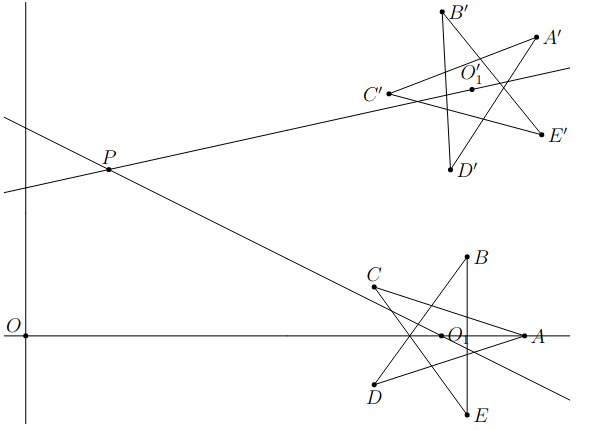
\includegraphics[width = 12cm]{estrella1.png}
\end{figure}

\textcolor{blue}{Dibujar dicha estrella así como su girada, mostrando además los segmentos $PO_1$ y $PO'_1$. Además calcular los siguientes puntos y valores:
\begin{enumerate} 
\item[a)] La ecuación de la recta $PO_1$.
\item[b)] La distancia de $A$ a la recta $PO_1$
\item[c)] Las coordenadas del punto $B$.
\item[d)] Las coordenadas del punto $O'_1$ centro de la estrella girada.
\item[e)] Las coordenadas del punto $B'$, vértice correspondiente con el vértice $B$ de la estrella girada.
\end{enumerate}}

\end{ejer}

{\it Solución:}

% Inicio del Ejercicio 6

Introducimos el sistema de referencia canónico con punto (5,0) y base $e_1,e_2$, $R$:
\begin{sageblock}
R = matrix(RR,[[1,0,0],
            [5,1,0],
            [0,0,1]])
R.subdivide(1,1)
\end{sageblock}
$$R=\sage{R}$$
El sistema de referencia para realizar el giro y obtener las estrella de vértices $A, B, C, D$ y $E$ será $g$. Para obtener los vértices de la estrella, definimos el ángulo $\beta = 2\pi/5$ y la matriz del giro de ángulo $\beta$ en este sistema de referencia
\begin{sageblock}
beta = 2*pi/5
G = matrix(RR,[[1, 0     ,  0      ],
            [0, cos(beta), -sin(beta)],
            [0, sin(beta),  cos(beta)]])
g=R*G*R^-1
g.subdivide(1,1)
\end{sageblock}

La matriz del giro del sistema de referencia que resulta es \[g=RG_{\frac{2 \pi}{5}}R^{-1} = \sage{g}.\]
Definimos los vértices del pentágono girando el vértice $A = \left( \begin{array}{r} 6  \\ 0 \end{array} \right)$ en coordenadas homogéneas

\begin{sageblock}
V = [g^i*vector(RR,[1,6,0]) for i in range(5)]
\end{sageblock}
Los vértices con coordenada homogénea son:
$$V[0]=(1,6,0)=\sage{V[0]}$$
$$V[1]=g(1,6,0)=\sage{V[1]}$$
$$V[2]=g^2(1,6,0)=\sage{V[2]}$$
$$V[3]=g^3(1,6,0)=\sage{V[3]}$$
$$V[4]=g^4(1,6,0)=\sage{V[4]}$$
Ahora debemos girar dichos vértices un ángulo de $39^\circ$ centrado en el punto $P = (1,2)$. Para eso introducimos como $R_1$ el sistema de referencia canónico en $P$.

\begin{sageblock}
R1 = matrix(RR,[[1,0,0],
             [1,1,0],
             [2,0,1]])
R1.subdivide(1,1)
\end{sageblock}

Nuestro sistema de referencia ahora es \[ R_1=\sage{R1} \] Definimos el ángulo $\alpha = 39\pi/180$ y la matriz del giro de ángulo $\alpha$ en este sistema de referencia 
\begin{sageblock}
alpha = 39*pi/180
G1 = matrix(RR,[[1, 0        ,  0        ],
            [0, cos(alpha), -sin(alpha)],
            [0, sin(alpha),  cos(alpha)]])
g1=R1*G1*R1^-1
g1.subdivide(1,1)
\end{sageblock}

La matriz del giro que resulta es \[g_1=R_1G_{\frac{39 \pi}{180}}R_1^{-1} = \sage{g1}.\] 
Los vértices en coordenadas homogéneas de la estrella girada con centro en el punto $P$ son

\begin{sageblock}
V1 = [g1*v for v in V]
\end{sageblock}
$$V_1[0]=g_1(1,6,0)=\sage{V1[0]}$$
$$V_1[1]=g_1(g(1,6,0))=\sage{V1[1]}$$
$$V_1[2]=g_1(g^2(1,6,0))=\sage{V1[2]}$$
$$V_1[3]=g_1(g^3(1,6,0))=\sage{V1[3]}$$
$$V_1[4]=g_1(g^4(1,6,0))=\sage{V1[4]}$$
Quitamos la coordenada homogénea para poder representar los puntos en el plano

\begin{sageblock}
V = [v[1:] for v in V]
V1 = [v[1:] for v in V1]
\end{sageblock}
De esta forma los puntos ahora son
Dibujamos las estrellas así como los puntos $P$, $O1$, $O'1$ y los segmentos $PO_1$ y $PO'_1$.
$$V[0]=\sage{V[0]} \quad V_1[0]=\sage{V1[0]}$$
$$V[1]=\sage{V[1]} \quad V_1[1]=\sage{V1[1]}$$
$$V[2]=\sage{V[2]} \quad V_1[2]=\sage{V1[2]}$$
$$V[3]=\sage{V[3]} \quad V_1[3]=\sage{V1[3]}$$
$$V[4]=\sage{V[4]} \quad V_1[4]=\sage{V1[4]}$$

Para introducir los comandos en Sagesub adecuadamente debemos introducir los siguientes puntos y vectores:
\begin{sageblock}
P=vector(RR,[1,2])
O1=vector(RR,[5,0])
g1O1=g1*vector(RR,[1,5,0])
g1O1=g1O1[1:]
\end{sageblock}
$$P=\sage{P}$$
$$O_1=\sage{O1}$$
$$g_1(O_1)=\sage{g1O1}$$
Introduciendo los siguientes comandos:
\begin{verbatim}
\begin{sagesub}
\begin{center}
\begin{tikzpicture}[scale = 1.3,
cara1/.style={thick, color = blue, fill opacity = 0.3, fill = blue!20},
cara2/.style={thick, color = red, fill opacity = 0.3, fill = red!20}]
\draw[->,thick,gray] (-1,0) -- (7,0); % Eje X
\draw[->,thick,gray] (0,-1) -- (0,5); % Eje Y
\draw[cara1] !{V[0]} -- !{V[2]} -- !{V[4]} -- !{V[1]} -- !{V[3]} -- cycle;
\draw[cara2] !{V1[0]} -- !{V1[2]} -- !{V1[4]} -- !{V1[1]} -- !{V1[3]} -- cycle;
\draw[dashed] !{P} -- !{O1};
\draw[dashed] !{P} -- !{g1O1};
\draw[fill = white] !{P} circle (0.5mm);
\draw[fill = white] !{P} circle (0.5mm) node[above left] {$P$};  
\draw[fill = white] !{O1} circle (0.5mm); 
\draw[fill = white] !{g1O1} circle (0.5mm); 
\end{tikzpicture}
\end{center}
\end{sagesub}
\end{verbatim}
se obtiene:

%%%%%%%%%%
%%dibujosagesub%%
%%%%%%%%%%%

\begin{sagesub}
\begin{center}
\begin{tikzpicture}[scale = 1.3,
cara1/.style={thick, color = blue, fill opacity = 0.3, fill = blue!20},
cara2/.style={thick, color = red, fill opacity = 0.3, fill = red!20}]
\draw[->,thick,gray] (-1,0) -- (7,0); % Eje X
\draw[->,thick,gray] (0,-1) -- (0,5); % Eje Y
\draw[cara1] !{V[0]} -- !{V[2]} -- !{V[4]} -- !{V[1]} -- !{V[3]} -- cycle;
\draw[cara2] !{V1[0]} -- !{V1[2]} -- !{V1[4]} -- !{V1[1]} -- !{V1[3]} -- cycle;
\draw[dashed] !{P} -- !{O1};
\draw[dashed] !{P} -- !{g1O1};
\draw[fill = white] !{P} circle (0.5mm);
\draw[fill = white] !{P} circle (0.5mm) node[above left] {$P$};  
\draw[fill = white] !{O1} circle (0.5mm); 
\draw[fill = white] !{g1O1} circle (0.5mm); 
\end{tikzpicture}
\end{center}
\end{sagesub}



Además

\begin{enumerate} 
\item[a)] Ecuación de la recta $PO_1$.

\begin{sageblock}
Pol.<x,y> = PolynomialRing(RR)
A=matrix(Pol,[[1,1,1],
            [x,1,5],
            [y,2,0]])
\end{sageblock}

La ecuación de la recta $PO_1$ es
\[ \left| \begin{array}{rrr}
1 & 1 & 1  \\            
x & 1 & 5  \\          
y & 2 & 0            
\end{array} \right| = 0\] Por tanto \[ \sage{det(A)} = 0 \] o equivalentemente \[ x + 2y - 5 = 0 \]

\item[b)] Distancia de $A$ a la recta $PO_1$


La distancia del punto $A = (6,0)$ sobre la recta $x+2y-5=0$ por tanto es \[ \frac{\vert 6\cdot 1+2\cdot 0-5\vert}{\sqrt{1^2+2^2}} = \frac{1}{\sqrt{5}} \]


\item[c)] Coordenadas del punto $B$.

Las coordenadas del punto $B$ son
\begin{sageblock}
B=g*vector(RR,[1,6,0])
B=B[1:]
\end{sageblock}
\[ \sage{n(B)} \] Obtendríamos el mismo resultado tomando $B=V[1]$.

\item[d)] Las coordenadas del punto $O'_1$ centro de la estrella girada.
 
\begin{sageblock}
g1O1=g1*vector(RR,[1,5,0])
g1O1=g1O1[1:]
\end{sageblock}
Las coordenadas del punto $O'_1$ son
\[ O'_1 = \sage{n(g1O1)} \]

\item[e)] Las coordenadas del punto $B'$, vértice correspondiente con el vértice $B$ de la estrella girada.

\begin{sageblock}
Bp=g1*g*vector(RR,[1,6,0])
Bp=Bp[1:]
\end{sageblock}

Las coordenadas del punto $B'$ son
\[ B' = \sage{n(Bp)} \] Obtendríamos el mismo resultado tomando $B'=V_1[1]$.

\end{enumerate}

% Fin del Ejercicio 6
\newpage

\begin{ejer}
\textcolor{blue}{Determina una estrella regular de $5$ puntas con centro en el punto $O_1 = (2,-3)$ y con vértice $A = (3,-2)$. El resto de los vértices se nombran $B, C, D$ y $E$ tal y como indica la figura. Posteriormente se hace una simetría ortogonal respecto de la recta que pasa por los puntos $P = (-2,7)$ y $Q = (0,9)$.}

\begin{figure}[H]
\centering
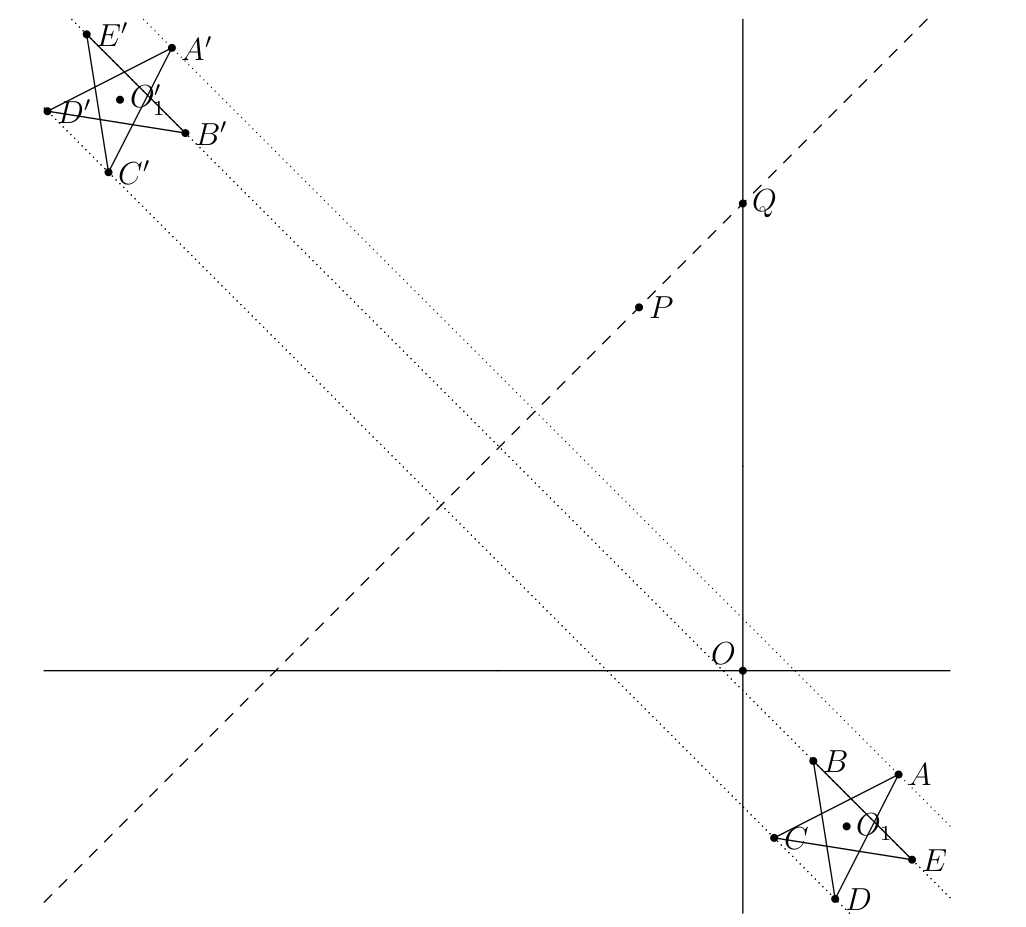
\includegraphics[width = 10cm]{estrella2.png}
\end{figure}

\textcolor{blue}{Dibujar dicha estrella así como su simétrica, mostrando además la recta que une los puntos $P$ y $Q$. Además calcular los siguientes puntos y valores:
\begin{enumerate} 
\item[a)] La ecuación de la recta $PQ$.
\item[b)] La distancia de $A$ a la recta $PQ$
\item[c)] Las coordenadas del punto $B$.
\item[d)] Las coordenadas del punto $O'_1$ centro de la estrella simétrica a la dada.
\item[e)] Las coordenadas del punto $B'$, vértice correspondiente con el vértice $B$ de la estrella simétrica.
\end{enumerate}}

\end{ejer}

{\it Solución:}
% Inicio del Ejercicio 7

El sistema de referencia para realizar el giro y obtener las estrella de vértices $A, B, C, D$ y $E$, es el que tiene como punto $O_1$ y base canónica $e_1,e_2$.
\begin{sageblock}
R = matrix(RR,[[ 1,0,0],
            [ 2,1,0],
            [-3,0,1]])
R.subdivide(1,1)
\end{sageblock}

 \[R= \sage{R} \]
Para obtener los vértices de la estrella, definimos el ángulo $\beta = 2\pi/5$ y la matriz del giro de ángulo $\beta$ en este sistema de referencia

\begin{sageblock}
beta = 2*pi/5
G = matrix(RR,[[1, 0        ,  0        ],
            [0, cos(beta), -sin(beta)],
            [0, sin(beta),  cos(beta)]])
g=R*G*R^-1
g.subdivide(1,1)
\end{sageblock}

La matriz del giro en sistema de referencia que resulta es \[g=RG_{\frac{2\pi}{5}} R^{-1}= \sage{g}.\]
Definimos los vértices en homogéneas del pentágono girando el vértice $A = \left( \begin{array}{r} 3  \\ -2 \end{array} \right)$
$$V=\{(1,3,-2), \ g(1,3,-2), \ g^2(1,3,-2), \ g^3(1,3,-2), \ g^4(1,3,-2) \}$$

\begin{sageblock}
V = [g^i*vector(RR,[1,3,-2]) for i in range(5)]
\end{sageblock}
$$V[0]=\sage{V[0]}$$
$$V[1]=\sage{V[1]}$$
$$V[2]=\sage{V[2]}$$
$$V[3]=\sage{V[3]}$$
$$V[4]=\sage{V[4]}$$
Ahora debemos determinar la simetría respecto de la recta que pasa por los puntos $P$ y $Q$ para obtener los vértices simétricos de los ya calculados.

Para ello tomamos como sistema de referencia un punto cualquiera de la recta junto con una base adecuada. Tomamos como punto, por ejemplo, $$P = (-2,7).$$ El primer vector de la base lo tomamos sobre la recta, por ejemplo, $$v_1 = \vec{PQ}= (0,9) - (-2,7) = (2,2)$$ y el segundo vector un ortogonal, por ejemplo $$v_2 = (-2,2).$$

\begin{sageblock}
P=vector(RR,[-2,7])
Q=vector(RR,[0,9])
v1 = Q-P
v2=vector(RR,[-v1[1],v1[0]])
R=block_matrix(RR,[[       matrix([1,0,0])],
                [column_matrix([P,v1,v2])]])
R.subdivide(1,1)
\end{sageblock}

El sistema de referencia es \[ R = \sage{R} \]
Introducimos la matriz de simetría:
\begin{sageblock}
sRR = matrix(RR,[[1,0, 0],
              [0,1, 0],
              [0,0,-1]])
sRR.subdivide(1,1)
s=R*sRR*R^-1
s.subdivide(1,1)
\end{sageblock}

Respecto de dicho sistema de referencia la matriz de la simetría es \[ S_{RR} = \sage{sRR} \] Y respecto del sistema canónico es la matriz \[ s = RS_{RR}R^{-1} = \sage{s} \]

Los vértices de la estrella simétrica son
$$V=\{s(1,3,-2), \ s(g(1,3,-2)), \ s(g^2(1,3,-2)), \ s(g^3(1,3,-2)), \ s(g^4(1,3,-2)) \}$$
\begin{sageblock}
V1 = [s*v for v in V]
\end{sageblock}
$$V_1[0]=\sage{V1[0]}$$
$$V_1[1]=\sage{V1[1]}$$
$$V_1[2]=\sage{V1[2]}$$
$$V_1[3]=\sage{V1[3]}$$
$$V_1[4]=\sage{V1[4]}$$
Quitamos la coordenada homogénea para poder representar los puntos en el plano

\begin{sageblock}
V = [vector(v[1:]) for v in V]
V1 = [vector(v[1:]) for v in V1]
\end{sageblock}
$$V[0]=\sage{V[0]} \quad V_1[0]=\sage{V1[0]}$$
$$V[1]=\sage{V[1]} \quad V_1[1]=\sage{V1[1]}$$
$$V[2]=\sage{V[2]} \quad V_1[2]=\sage{V1[2]}$$
$$V[3]=\sage{V[3]} \quad V_1[3]=\sage{V1[3]}$$
$$V[4]=\sage{V[4]} \quad V_1[4]=\sage{V1[4]}$$
Dibujamos las estrellas así como los puntos $P$ y $Q$, el segmento que los une y los centros $O_1$ y $O'_1$.

\begin{sageblock}
O1=vector(RR,[2,-3])
sO1=s*vector(RR,[1,2,-3])
sO1=sO1[1:]
\end{sageblock}
De esta forma,
$$O_1=\sage{O1}$$
$$O'_1=s(O_1)=\sage{sO1}$$
Obteniendo:

\begin{sagesub}
\begin{center}
\begin{tikzpicture}[scale = 0.5,
cara1/.style={thick, color = blue, fill opacity = 0.3, fill = blue!20},
cara2/.style={thick, color = red, fill opacity = 0.3, fill = red!20}]
\draw[->,thick,gray] (4.5,0) -- (-14,0); % Eje X
\draw[->,thick,gray] (0,-5) -- (0,14); % Eje Y
\draw[cara1] !{V[0]} -- !{V[2]} -- !{V[4]} -- !{V[1]} -- !{V[3]} -- cycle;
\draw[cara2] !{V1[0]} -- !{V1[2]} -- !{V1[4]} -- !{V1[1]} -- !{V1[3]} -- cycle;
\draw[dashed] (-9,0) -- (2,11);
\draw[dashed] !{O1} -- !{sO1};
\draw[fill = white] !{P} circle (0.5mm);
\draw[fill = white] !{Q} circle (0.5mm);
\draw[fill = white] !{P} circle (0.5mm) node[above left] {$P$}; 
\draw[fill = white] !{Q} circle (0.5mm) node[above left] {$Q$};  
\draw[fill = white] !{O1} circle (0.5mm); 
\draw[fill = white] !{sO1} circle (0.5mm); 
\end{tikzpicture}
\end{center}
\end{sagesub}

El código que hay tras el dibujo es el siguiente:
%%%%%%
%%dibujosagesub
%%%%%%
\begin{verbatim}
\begin{sagesub}
\begin{center}
\begin{tikzpicture}[scale = 0.5,
cara1/.style={thick, color = blue, fill opacity = 0.3, fill = blue!20},
cara2/.style={thick, color = red, fill opacity = 0.3, fill = red!20}]
\draw[->,thick,gray] (4.5,0) -- (-14,0); % Eje X
\draw[->,thick,gray] (0,-5) -- (0,14); % Eje Y
\draw[cara1] !{V[0]} -- !{V[2]} -- !{V[4]} -- !{V[1]} -- !{V[3]} -- cycle;
\draw[cara2] !{V1[0]} -- !{V1[2]} -- !{V1[4]} -- !{V1[1]} -- !{V1[3]} -- cycle;
\draw[dashed] (-9,0) -- (2,11);
\draw[dashed] !{O1} -- !{sO1};
\draw[fill = white] !{P} circle (0.5mm);
\draw[fill = white] !{Q} circle (0.5mm);
\draw[fill = white] !{P} circle (0.5mm) node[above left] {$P$}; 
\draw[fill = white] !{Q} circle (0.5mm) node[above left] {$Q$};  
\draw[fill = white] !{O1} circle (0.5mm); 
\draw[fill = white] !{sO1} circle (0.5mm); 
\end{tikzpicture}
\end{center}
\end{sagesub}
\end{verbatim}
Además

\begin{enumerate} 
\item[a)] Ecuación de la recta $PQ$.

\begin{sageblock}
Pol.<x,y>=PolynomialRing(RR)
A=matrix(Pol,[[1,1,1],
            [x,-2,0],
            [y,7,9]])
\end{sageblock}

La ecuación de la recta $PQ$ es
\[ \left| \begin{array}{rrr}
1 & 1 & 1  \\            
x & -2 & 0  \\          
y & 7 & 9            
\end{array} \right| = 0\] Por tanto \[ \sage{det(A)} = 0 \] o equivalentemente \[ -x + y - 9 = 0 \]

\item[b)] Distancia de $A$ a la recta $PQ$

La distancia del punto $A = (3,-2)$ sobre la recta $-x+y-9=0$ por tanto es \[ \frac{\vert -(3)+ (-2)-9\vert}{\sqrt{(-1)^2+1^2}} = \frac{14}{\sqrt{2}}=7\sqrt{2} \]


\item[c)] Coordenadas del punto $B$.

Las coordenadas del punto $B$ son
\begin{sageblock}
B=g*vector(RR,[1,3,-2])
B=B[1:]
\end{sageblock}
\[ B=\sage{n(B)} \] Obtendríamos el mismo resultado tomando $B=V[1]$.

\item[d)] Las coordenadas del punto $O'_1$ centro de la estrella simétrica a la dada.
 
\begin{sageblock}
sO1=s*vector(RR,[1,2,-3])
sO1=sO1[1:]
\end{sageblock}
Las coordenadas del punto $O'_1$ son
\[ O'_1 = \sage{n(sO1)} \] 

\item[e)] Las coordenadas del punto $B'$, vértice correspondiente con el vértice $B$ de la estrella simétrica.

\begin{sageblock}
Bp=s*g*vector(RR,[1,3,-2])
Bp=Bp[1:]
\end{sageblock}

Las coordenadas del punto $B'$ son
\[ B' = \sage{n(Bp)} \] Obtendríamos el mismo resultado tomando $B'=V_1[1]$.


\end{enumerate}
% Fin del Ejercicio 7

\newpage

\begin{ejer}
\textcolor{blue}{Calcula la matriz de la transformación afín que corresponde a la simetría ortogonal con respecto al plano que pasa por los puntos $A = \left[ \begin{array}{r} 1 \\ 2 \\ -1 \end{array} \right]$, $B = \left[ \begin{array}{r} 2 \\ 1 \\ 1 \end{array} \right]$ y $C = \left[ \begin{array}{r} -1 \\ 3 \\ 1 \end{array} \right]$.}
\end{ejer}

{\it Solución:}
% Inicio del Ejercicio 8

\begin{sageblock}
A = vector(RR, [1, 2, -1])
B = vector(RR, [2, 1, 1])
C = vector(RR, [-1, 3, 1])

AB = B - A
AC = C - A
n = AB.cross_product(AC)

u1 = AB.normalized()
u2 = n.cross_product(AB)
u3 = n.normalized()

R = block_matrix(2, 1, [matrix(RR, [1, 0, 0, 0]), column_matrix([A, u1, u2, u3])])
R.subdivide(1, 1)

MRRs = matrix(RR, [[1, 0, 0, 0], [0, 1, 0, 0], [0, 0, 1, 0], [0, 0, 0, -1]])

Ms = R * MRRs * R^-1
Ms.subdivide(1, 1)
\end{sageblock}

$$
	M_s = \sage{Ms}
$$

% Fin del Ejercicio 8

\newpage

\begin{ejer}
\textcolor{blue}{Calcula la matriz de la homotecia con factor $\frac{1}{2}$ y con centro en el punto $\left[ \begin{array}{r} -2 \\ 2 \\ 1 \end{array} \right]$}
\end{ejer}

{\it Solución:}

% Inicio del Ejercicio 9

\begin{sageblock}
R = matrix(RR, [[1, 0, 0, 0], [-2, 1, 0, 0], [2, 0, 1, 0], [1, 0, 0, 1]])
f = 1/2
MRRh = matrix(RR, [[1, 0, 0, 0], [0, f, 0, 0], [0, 0, f, 0], [0, 0, 0, f]])
Mh = R * MRRh * R^-1
Mh.subdivide(1, 1)
\end{sageblock}

$$
	M_h = \sage{Mh}
$$
% Fin del Ejercicio 9


\newpage

\begin{ejer}
\textcolor{blue}{Calcula los vértices de un heptágono regular en $\mathcal{A}^3(\mathbb{R})$, sabiendo que 
están contenidos en el plano $3x+y-z=1$, que su centro está en el punto $P=\left[\begin{array}{c}1\\0\\2
\end{array}\right]$, y que uno de dichos vértices es el punto $Q=\left[\begin{array}{c}1\\1\\3
\end{array}\right]$.}
\end{ejer}

{\it Solución.-}

% Inicio del Ejercicio 10
\begin{sageblock}
n = vector(RR, [3, 1, -1])
P = vector(RR, [1, 0, 2])
Q = vector(RR, [1, 1, 3])

PQ = Q - P

u1 = PQ.normalized()
u2 = PQ.cross_product(n).normalized()
u3 = n.normalized()

R = block_matrix(2, 1, [matrix(RR, [1, 0, 0, 0]), column_matrix([P, u1, u2, u3])])
R.subdivide(1, 1)

a = 2*pi/7
MRRg = matrix(RR, [[1, 0, 0, 0], [0, cos(a), -sin(a), 0], [0, sin(a), cos(a), 0], [0, 0, 0, 1]])

Mg = R * MRRg * R^-1

C = [Mg^i * vector(RR, [1, 1, 1, 3]) for i in range(7)]
W = [v[1:] for v in C]
\end{sageblock}

\begin{sagesub}
\begin{center}
\tdplotsetmaincoords{70}{110}
\begin{tikzpicture}[scale = 1, tdplot_main_coords,
cara/.style={thick, color = blue, fill opacity = 0.3, fill = blue!20}]
\draw[->,thick,gray] (-5,0,0) -- (5,0,0); % Eje X
\draw[->,thick,gray] (0,-5,0) -- (0,5,0); % Eje Y
\draw[->,thick,gray] (0,0,-1) -- (0,0,5); % Eje Z
\draw[cara] !{W[0]} -- !{W[1]} -- !{W[2]} -- !{W[3]} -- !{W[4]} -- !{W[5]}
-- !{W[6]} -- cycle;
\draw[cara] !{P+3*u1+3*u2} -- !{P+3*u1-3*u2} -- !{P-3*u1-3*u2} -- !{P-3*u1+3*u2} -- cycle;
\draw[black] (1, 1, 3) circle (2pt);
\draw[black] (1, 0, 2) circle (2pt);
\end{tikzpicture}
\end{center}
\end{sagesub}
% Fin del Ejercicio 10

\newpage


\begin{ejer}
\textcolor{blue}{Calcula el simétrico de cada uno de los puntos
$$
	\left[\begin{array}{c}1\\1\\0\end{array}\right] \quad
	\left[\begin{array}{c}2\\-1\\-3\end{array}\right] \quad
	\left[\begin{array}{c}3\\3\\-1\end{array}\right] \quad
	\left[\begin{array}{c}2\\3\\1\end{array}\right] \quad
	\left[\begin{array}{c}4\\-6\\10\end{array}\right] \quad
	\left[\begin{array}{c}5\\10\\-15\end{array}\right]
$$ 
respecto del plano $x+y=1$. Dibuja todos los puntos, sus simétricos y el plano.}
\end{ejer}

{\it Solución:}

% Inicio del Ejercicio 11
\begin{sageblock}
D = vector(RR, [1, 1, 1, 0]), vector(RR, [1, 2, -1, -3]), vector(RR, [1, 3, -3, -1]), vector(RR, [1, 2, 3, 1]), vector(RR, [1, 4, -6, 10]), vector(RR, [1, 5, 10, -15])

n = vector(RR, [1, 1, 0])
v1 = vector(RR, [-n[1], n[0], 0])
v2 = n.cross_product(v1)

u1, u2, u3 = v1.normalized(), v2.normalized(), n.normalized()

# x = 0, y = 1
R = block_matrix(2, 1, [matrix(RR, [1, 0, 0, 0]), column_matrix(RR, [vector(RR, [0, 1, 0]), u1, u2, u3])])

MRRs = matrix(RR, [[1, 0, 0, 0], [0, 1, 0, 0],  [0, 0, 1, 0], [0, 0, 0, -1]])

Ms = R * MRRs * R^-1

sime = [Ms * v for v in D]
\end{sageblock}

El código que hay tras el dibujo es:

$$
\sage{Ms}
$$

\begin{sagesub}
\begin{center}
\tdplotsetmaincoords{70}{110}
\begin{tikzpicture}[scale = 0.3, tdplot_main_coords,
  cara/.style={thick, color = blue, fill opacity = 0.3, fill = blue!20}]
\draw[->,thick,gray] (-15,0,0) -- (15,0,0); % Eje X
\draw[->,thick,gray] (0,-15,0) -- (0,15,0); % Eje Y
\draw[->,thick,gray] (0,0,-15) -- (0,0,15); % Eje Z
\draw[->,thick,gray] (0,0,0) -- !{5*u1} node[below right] {$u_1$};
\draw[->,thick,gray] (0,0,0) -- !{5*u2} node[below right] {$u_2$};
\draw[->,thick,gray] (0,0,0) -- !{5*u3} node[below right] {$u_3$};
\draw[fill = blue] !{D[0]} circle (2mm) node[above left] {$P_1$}; 
\draw[fill = blue] !{D[1]} circle (2mm) node[below right] {$P_2$}; 
\draw[fill = blue] !{D[2]} circle (2mm) node[below right] {$P_3$}; 
\draw[fill = blue] !{D[3]} circle (2mm) node[above right] {$P_4$}; 
\draw[fill = blue] !{D[4]} circle (2mm) node[above right] {$P_5$}; 
\draw[fill = blue] !{D[5]} circle (2mm) node[above right] {$P_6$}; 
\draw[fill = red] !{sime[0]} circle (2mm) node[above left] {$P'_1$}; 
\draw[fill = red] !{sime[1]} circle (2mm) node[below right] {$P'_2$}; 
\draw[fill = red] !{sime[2]} circle (2mm) node[below right] {$P'_3$}; 
\draw[fill = red] !{sime[3]} circle (2mm) node[above right] {$P'_4$}; 
\draw[fill = red] !{sime[4]} circle (2mm) node[above right] {$P'_5$}; 
\draw[fill = red] !{sime[5]} circle (2mm) node[above right] {$P'_6$}; 
\draw[cara] !{16*u1+16*u2} -- !{16*u1-16*u2} -- !{-16*u1-16*u2} -- !{-16*u1+16*u2} -- cycle;
\end{tikzpicture}
\end{center}
\end{sagesub}

% Fin del Ejercicio 11

\newpage


\begin{ejer}
\textcolor{blue}{Sabiendo que la simetría ortogonal $f:\mathcal{A}^3(\mathbb{R}) \to \mathcal{A}^3(\mathbb{R})$
respecto a un cierto plano cumple 
$$
	f\left(\left[\begin{array}{c}1\\3\\-1\end{array}\right]\right)=\left[\begin{array}{c}3\\2\\1\end{array}\right],
$$ 
calcula un sistema de referencia af\'in de dicho plano y la matriz de~$f$ respecto del sistema de referencia can\'onico
de $\mathcal{A}^3(\mathbb{R})$. }
\end{ejer}
{\it Solución:}

% Inicio del Ejercicio 12

Calcular plano

\begin{sageblock}
A = vector(RR, [1, 3, -1])
B = vector(RR, [3, 2, 1])
AB = B - A
PM = A + (AB / 2)

n = AB
v1 = vector(RR, [-n[1], n[0], 0])
v2 = n.cross_product(v1)


u1 = v1.normalized()
u2 = v2.normalized()
u3 = n.normalized()

R = block_matrix(2, 1, [matrix(RR, [1, 0, 0, 0]), column_matrix([PM, u1, u2, u3])])

MRRs = matrix(RR, [[1, 0, 0, 0], [0, 1, 0, 0], [0, 0, 1, 0], [0, 0, 0, -1]])

Ms = R * MRRs * R^-1
\end{sageblock}

$$
\sage{Ms}
$$

\begin{sagesub}
\begin{center}
\tdplotsetmaincoords{70}{110}
\begin{tikzpicture}[scale = 1, tdplot_main_coords,
cara/.style={thick, color = blue, fill opacity = 0.3, fill = blue!20}]
\draw[->,thick,gray] (-5,0,0) -- (5,0,0); % Eje X
\draw[->,thick,gray] (0,-5,0) -- (0,5,0); % Eje Y
\draw[->,thick,gray] (0,0,-5) -- (0,0,5); % Eje Z
\draw[->,thick,red] !{PM} -- !{PM+2*u1} node[below right] {$u_1$};
\draw[->,thick,red] !{PM} -- !{PM+2*u2} node[below right] {$u_2$};
\draw[->,thick,red] !{PM} -- !{PM+2*u3} node[below right] {$u_3$};
\draw[fill = blue] !{A} circle (1mm) node[above left] {$A$}; 
\draw[fill = blue] !{B} circle (1mm) node[below right] {$B$};
\draw[fill = blue] !{PM} circle (1mm) node[below right] {$PM$}; 
\end{tikzpicture}
\end{center}
\end{sagesub}

% Fin del Ejercicio 12

\newpage


\begin{ejer}\label{ej:prisma}
\textcolor{blue}{Dibuja un prisma en $\mathcal{A}^3(\mathbb{R})$ con centro de gravedad el origen de coordenadas y bases pentagonales regulares en planos paralelos al plano $\Pi \equiv x+y+2z=0$, y que tenga al punto $A=\left[\begin{array}{c}0.5\\0.1\\0.4\end{array}\right]$ como uno de sus v\'ertices.} 
\end{ejer}

{\it Solución:}

% Inicio del Ejercicio 13

\begin{sageblock}
# plano
pn = vector(RR, [1, 1, 2])
v1 = vector(RR, [-pn[1], pn[0], 0])
v2 = pn.cross_product(v1)

A = vector(RR, [0.5, 0.1, 0.4])
Ah = vector(RR, [1, 00.5, 0.1, 0.4])

# proyectar A en la normal del plano obteniendo centro de cara
u1, u2, u3 = pn.normalized(), v1.normalized(), v2.normalized()
pB = column_matrix([u1, u2, u3])
MBBpv = matrix(RR, [[1, 0, 0], [0, 0, 0], [0, 0, 0]])
Mpn = pB * MBBpv * pB^-1
cO = Mpn * A

# rotar A en el centro de la cara obteniendo puntos de cara
cR = block_matrix(2, 1, [matrix(RR, [1, 0, 0, 0]), column_matrix([cO, u2, u3, u1])])
a = 2*pi/5
McRcRr = matrix(RR, [[1, 0, 0, 0], [0, cos(a), -sin(a), 0], [0, sin(a), cos(a), 0], [0, 0, 0, 1]])
Mcr = cR * McRcRr * cR^-1
cAP = [Mcr^i * Ah for i in range(5)]
cAP = [v[1:] for v in cAP]

# simetria de cara por el plano obteniendo la otra cara
MBBsp = matrix(RR, [[-1, 0, 0], [0, 1, 0], [0, 0, 1]])
Msp = pB * MBBsp * pB^-1
cBP = [Msp * v for v in cAP]
\end{sageblock}


\begin{sagesub}
\begin{center}
\tdplotsetmaincoords{70}{110}
\begin{tikzpicture}[scale = 5, tdplot_main_coords,
  cara/.style={thick, color = blue, fill opacity = 0.3, fill = blue!20},
  cara2/.style={thick, color = purple, fill opacity = 0.2, fill = purple!20},
  ]
\draw[->,thick,gray] (-1.5,0,0) -- (2.5,0,0); % Eje X
\draw[->,thick,gray] (0,-1.5,0) -- (0,1.5,0); % Eje Y
\draw[->,thick,gray] (0,0,-1.5) -- (0,0,1.5); % Eje Z
\draw[->,thick,red] (0, 0, 0) -- !{0.5*u1} node[below right] {$u_1$};
\draw[->,thick,red] (0, 0, 0) -- !{0.5*u2} node[below right] {$u_2$};
\draw[->,thick,red] (0, 0, 0) -- !{0.5*u3} node[below right] {$u_3$};
\draw[->,thick,green] !{cO} -- !{cO + 0.5*u2} node[below right] {$r_1$};
\draw[->,thick,green] !{cO} -- !{cO + 0.5*u3} node[below right] {$r_2$};
\draw[->,thick,green] !{cO} -- !{cO + 0.5*u1} node[below right] {$r_3$};
\draw[cara2] !{-0.5*u2 -0.5*u3} -- !{0.5*u2 -0.5*u3} -- !{0.5*u2 +0.5*u3} -- !{-0.5*u2 +0.5*u3} -- cycle;

\draw[cara] !{cAP[0]} -- !{cAP[1]} -- !{cAP[2]} -- !{cAP[3]} -- !{cAP[4]} -- cycle;
\draw[cara] !{cBP[0]} -- !{cBP[1]} -- !{cBP[2]} -- !{cBP[3]} -- !{cBP[4]} -- cycle;
\draw[cara] !{cAP[0]} -- !{cBP[0]} -- !{cBP[1]} -- !{cAP[1]} -- cycle;
\draw[cara] !{cAP[1]} -- !{cBP[1]} -- !{cBP[2]} -- !{cAP[2]} -- cycle;
\draw[cara] !{cAP[2]} -- !{cBP[2]} -- !{cBP[3]} -- !{cAP[3]} -- cycle;
\draw[cara] !{cAP[3]} -- !{cBP[3]} -- !{cBP[4]} -- !{cAP[4]} -- cycle;
\draw[cara] !{cAP[4]} -- !{cBP[4]} -- !{cBP[0]} -- !{cAP[0]} -- cycle;
\draw[fill = blue] !{A} circle (0.1mm) node[above left] {$A$};
\draw[fill = blue] !{cO} circle (0.1mm) node[above left] {$O_c$}; 
\end{tikzpicture}
\end{center}
\end{sagesub}

% Fin del Ejercicio 13


\newpage


\begin{ejer}
\textcolor{blue}{Calcula los vértices de una {\sc pirámide} $C \subseteq \mathcal{A}^3(\mathbb R)$ de altura $5$ cuya base 
sea un pentágono regular inscrito en una circunferencia de radio $1$ que esté contenido en el plano de ecuación $x-y+z=2$.} 
\end{ejer}

{\it Solución:}

% Inicio del ejercicio 14

Tomamos como punto base, un punto del plano $P = \left( \begin{array}{r} 1 \\ 0 \\ 1 \end{array} \right)$ y como base, una base $B = \{ v_1,v_2,v_3 \}$ donde $\{ v_1,v_2 \}$ sea una base ortonormal del espacio de dirección del plano y el vector $v_3$ un vector unitario ortogonal al plano.

\begin{sageblock}
P=vector(RR,[1,0,1])
v3 = vector(RR,[1,-1,1])
v1 = vector(RR,[1,1,0])
v2 = v1.cross_product(v3)
v1=v1/norm(v1)
v2=v2/norm(v2)
v3=v3/norm(v3)
\end{sageblock}

Sistema de referencia $R$:

\begin{sageblock}
R = block_matrix(RR,[[       matrix([1, 0, 0, 0])],
                     [column_matrix([P,v1,v2,v3])]])
R.subdivide(1,1)
\end{sageblock}

De donde \[ R = \sage{R}. \]

Para calcular los puntos de la base de la pirámide construimos la matriz del 
giro de ángulo $2\pi/5$ y la pasamos al nuevo sistema de referencia.
\begin{sageblock}
a = 2*pi/5
G = column_matrix(RR,[[1,    0,     0,  0],
                     [0,cos(a),sin(a), 0],
                     [0,-sin(a),cos(a),0],
                     [0,    0,     0,  1]])
g = R*G*R^-1
g.subdivide(1,1)
\end{sageblock}
$$g=RG_{\frac{2\pi}{5}}R^{-1}=\sage{g}$$
Los vértices de la pirámide, pentágono regular, está inscrito en una circunferencia de radio $1$. Nuestra base es ortonormal. Por tanto, $||v_1||=1$. Así que podemos suponer por tanto que el punto que debemos girar es aquel que tiene como coordenadas $[1,1,0,0]$ en el sistema de referencia $R$. Dicho punto en el sistema de referencia canónico es $$R*vector(RR,[1,1,0,0])$$  o equivalentemente el punto $P+v_1$.

Los puntos de la base de la pirámide serán los que corresponden a girar dicho punto cinco veces. 

\begin{sageblock}
puntogiro=R*vector(RR,[1,1,0,0])
BasePiramideh = [g^i*puntogiro for i in range(5)]
\end{sageblock}

El vértice de la pirámide, es el punto que tiene como coordenadas $[1,0,0,5]$ respecto del sistema de referencia $R$ (punto de altura $5$). Dicho punto en el sistema de referencia canónico es $$R*vector(RR,[1,0,0,5])$$

\begin{sageblock}
Verticeh = R*vector(RR,[1,0,0,5])
\end{sageblock}

Para poder dibujar la pirámide eliminamos la coordenada homogénea y unimos las aristas de la base y las que unen el vértice con los vértices de la base. Finalmente generamos el dibujo.

\begin{sageblock}
BP = [v[1:] for v in BasePiramideh]
Vertice = Verticeh[1:]
\end{sageblock}
Los vértices base de la pirámide son:
$$BP[0]=\sage{BP[0]}$$
$$BP[1]=\sage{BP[1]}$$
$$BP[2]=\sage{BP[2]}$$
$$BP[3]=\sage{BP[3]}$$
$$BP[4]=\sage{BP[4]}$$
Y el vértice de la pirámide es:
$$Vertice=\sage{Vertice}$$
Si ejecutamos el siguiente código de Sagesub:
\begin{verbatim}
\begin{sagesub}
\begin{center}
\tdplotsetmaincoords{70}{110}
\begin{tikzpicture}[scale = 1.6, tdplot_main_coords,
  cara/.style={thick, color = blue, fill opacity = 0.3, fill = blue!20},
  ]
\draw[->,thick,gray] (-2.5,0,0) -- (3.5,0,0); % Eje X
\draw[->,thick,gray] (0,-2.5,0) -- (0,2.5,0); % Eje Y
\draw[->,thick,gray] (0,0,-2.5) -- (0,0,2.5); % Eje Z
\draw[cara] !{BP[0]} -- !{BP[1]} -- !{BP[2]} -- !{BP[3]} -- !{BP[4]} --cycle;
\draw[cara] !{BP[0]} -- !{Vertice} -- !{BP[1]} -- cycle;
\draw[cara] !{BP[1]} -- !{Vertice} -- !{BP[2]} -- cycle;
\draw[cara] !{BP[2]} -- !{Vertice} -- !{BP[3]} -- cycle;
\draw[cara] !{BP[3]} -- !{Vertice} -- !{BP[4]} -- cycle;
\draw[cara] !{BP[4]} -- !{Vertice} -- !{BP[0]} -- cycle;
\end{tikzpicture}
\end{center}
\end{sagesub}
\end{verbatim}
obtenemos:
%%%%%%%%
%%dibujosagesub
%%%%%%%%%

\begin{sagesub}
\begin{center}
\tdplotsetmaincoords{70}{110}
\begin{tikzpicture}[scale = 1.6, tdplot_main_coords,
  cara/.style={thick, color = blue, fill opacity = 0.3, fill = blue!20},
  ]
\draw[->,thick,gray] (-2.5,0,0) -- (3.5,0,0); % Eje X
\draw[->,thick,gray] (0,-2.5,0) -- (0,2.5,0); % Eje Y
\draw[->,thick,gray] (0,0,-2.5) -- (0,0,2.5); % Eje Z
\draw[cara] !{BP[0]} -- !{BP[1]} -- !{BP[2]} -- !{BP[3]} -- !{BP[4]} --cycle;
\draw[cara] !{BP[0]} -- !{Vertice} -- !{BP[1]} -- cycle;
\draw[cara] !{BP[1]} -- !{Vertice} -- !{BP[2]} -- cycle;
\draw[cara] !{BP[2]} -- !{Vertice} -- !{BP[3]} -- cycle;
\draw[cara] !{BP[3]} -- !{Vertice} -- !{BP[4]} -- cycle;
\draw[cara] !{BP[4]} -- !{Vertice} -- !{BP[0]} -- cycle;
\end{tikzpicture}
\end{center}
\end{sagesub}

% Fin del Ejercicio 14

\newpage



\begin{ejer}
\textcolor{blue}{Calcula los vértices de una {\sc torre} $C \subseteq \mathcal{A}^3(\mathbb R)$ de altura $3$ cuya base 
sea un hexágono regular de lado $1$ que esté contenido en el plano de ecuación $2x-y+z=1$. }
\end{ejer}

{\it Solución.-}

% Escribe tu solución para el ejercicio 15


Para construir los vectores de la base, tomaremos $v_3$ el vector normal al plano y
$\{v_1, v_2\}$ una base ortonormal del espacio de direcciones del plano.

\begin{sageblock}
v3 = vector(RR,[2,-1,1])
v1 = vector(RR,[1,2,0])
v2 = v1.cross_product(v3)
v1=v1/norm(v1)
v2=v2/norm(v2)
v3=v3/norm(v3)
\end{sageblock}

El sistema de referencia que debemos tomar tiene como punto base, un punto del plano $P = \left( \begin{array}{r} 1 \\ 1 \\ 0 \end{array} \right)$ y como vectores los que hemos calculado, $v_1, v_2$ y $v_3$.

\begin{sageblock}
P = vector(RR,[1,1,0])
R = block_matrix(RR,[[       matrix([1, 0, 0, 0])],
                     [column_matrix([P,v1,v2,v3])]])
R.subdivide(1,1)
\end{sageblock}
$$R=\sage{R}$$
Para calcular los puntos de la base de la torre construimos la matriz del 
giro de ángulo $2\pi/6$ y la pasamos al nuevo sistema de referencia.
\begin{sageblock}
a = 2*pi/6
G = column_matrix(RR,[[1,    0,     0,  0],
                     [0,cos(a),sin(a), 0],
                     [0,-sin(a),cos(a),0],
                     [0,    0,     0,  1]])
g = R*G*R^-1
g.subdivide(1,1)
\end{sageblock}
$$g=RG_{\frac{2\pi}{6}}R^{-1}=\sage{g}$$
Los vértices de la base de la torre, hexágono regular, está inscrito en una circunferencia de radio $1$. Los hexágonos regulares tienen la propiedad de que la distancia del centro del hexágono a cualquier vértice del mismo mide lo mismo que la arista. Por lo tanto, podemos suponer por tanto que el punto que debemos girar es aquel que tiene como coordenadas $[1,1,0,0]$ en el sistema de referencia $R$. Dicho punto en el sistema de referencia canónico es $$R*vector(RR,[1,1,0,0])$$ o equivalentemente el punto $P+v_1$.
\begin{sageblock}
BaseTorreh = [g^i*R*vector(RR,[1,1,0,0]) for i in range(6)]
\end{sageblock} 
Los puntos de la base de la torre serán los que corresponden a girar el primero de los puntos seis veces.


Para obtener la tapa de la torre, sumamos a cada punto de la base de la torre el vector de coordenadas $[1,0,0,3]$ en el sistema de referencia $R$ (vector de altura $3$). Es decir le sumamos el vector
 $$R*vector[1,0,0,3]$$

\begin{sageblock}
TapaTorreh = [v+R*vector(RR,[1,0,0,3]) for v in BaseTorreh] 
\end{sageblock}

Seguidamente eliminamos la coordenada homogénea y unimos las aristas de la base, las aristas de la tapa además de las aristas laterales de la torre. Finalmente generamos el dibujo.

\begin{sageblock}
BT = [v[1:] for v in BaseTorreh]
TT = [w[1:] for w in TapaTorreh] 
\end{sageblock}
Podemos entonces introducir el siguiente código en sagesub:
\begin{verbatim}
\begin{sagesub}
\begin{center}
\tdplotsetmaincoords{70}{110}
\begin{tikzpicture}[scale = 2.4, tdplot_main_coords,
  cara/.style={thick, color = blue, fill opacity = 0.3, fill = blue!20},
  ]
\draw[->,thick,gray] (-2.5,0,0) -- (3.5,0,0); % Eje X
\draw[->,thick,gray] (0,-2.5,0) -- (0,2.5,0); % Eje Y
\draw[->,thick,gray] (0,0,-2.5) -- (0,0,2.5); % Eje Z
\draw[cara] !{BT[0]} -- !{BT[1]} -- !{BT[2]} -- !{BT[3]} -- !{BT[4]} -- !{BT[5]} --cycle;
\draw[cara] !{TT[0]} -- !{TT[1]} -- !{TT[2]} -- !{TT[3]} -- !{TT[4]} -- !{TT[5]} --cycle;
\draw[cara] !{BT[0]} -- !{TT[0]} -- !{TT[1]} -- !{BT[1]} -- cycle;
\draw[cara] !{BT[1]} -- !{TT[1]} -- !{TT[2]} -- !{BT[2]} -- cycle;
\draw[cara] !{BT[2]} -- !{TT[2]} -- !{TT[3]} -- !{BT[3]} -- cycle;
\draw[cara] !{BT[3]} -- !{TT[3]} -- !{TT[4]} -- !{BT[4]} -- cycle;
\draw[cara] !{BT[4]} -- !{TT[4]} -- !{TT[5]} -- !{BT[5]} -- cycle;
\draw[cara] !{BT[5]} -- !{TT[5]} -- !{TT[0]} -- !{BT[0]} -- cycle;
\end{tikzpicture}
\end{center}
\end{sagesub}
\end{verbatim}
para realizar el dibujo que nos piden:
%%%%%%%%%%
%%dibujosagesub%
%%%%%%%%%%%

\begin{sagesub}
\begin{center}
\tdplotsetmaincoords{70}{110}
\begin{tikzpicture}[scale = 2.4, tdplot_main_coords,
  cara/.style={thick, color = blue, fill opacity = 0.3, fill = blue!20},
  ]
\draw[->,thick,gray] (-2.5,0,0) -- (3.5,0,0); % Eje X
\draw[->,thick,gray] (0,-2.5,0) -- (0,2.5,0); % Eje Y
\draw[->,thick,gray] (0,0,-2.5) -- (0,0,2.5); % Eje Z
\draw[cara] !{BT[0]} -- !{BT[1]} -- !{BT[2]} -- !{BT[3]} -- !{BT[4]} -- !{BT[5]} --cycle;
\draw[cara] !{TT[0]} -- !{TT[1]} -- !{TT[2]} -- !{TT[3]} -- !{TT[4]} -- !{TT[5]} --cycle;
\draw[cara] !{BT[0]} -- !{TT[0]} -- !{TT[1]} -- !{BT[1]} -- cycle;
\draw[cara] !{BT[1]} -- !{TT[1]} -- !{TT[2]} -- !{BT[2]} -- cycle;
\draw[cara] !{BT[2]} -- !{TT[2]} -- !{TT[3]} -- !{BT[3]} -- cycle;
\draw[cara] !{BT[3]} -- !{TT[3]} -- !{TT[4]} -- !{BT[4]} -- cycle;
\draw[cara] !{BT[4]} -- !{TT[4]} -- !{TT[5]} -- !{BT[5]} -- cycle;
\draw[cara] !{BT[5]} -- !{TT[5]} -- !{TT[0]} -- !{BT[0]} -- cycle;
\end{tikzpicture}
\end{center}
\end{sagesub}

% Fin del Ejercicio 15





\end{document}
